\documentclass[12pt]{article}
\everymath{\displaystyle}
\usepackage{unicode-math}
\usepackage{pgfplots}
\pgfplotsset{compat=1.18}
\usepackage{amsmath}



\usepackage[margin=1in]{geometry}
\usepackage{tcolorbox}
\usepackage{graphicx}
\usepackage{tikz}
\usepackage{amssymb}
\usepackage{enumitem}
\usepackage{titlesec}
\usepackage{fancyhdr}
\usepackage{pifont}
\usepackage{xcolor}
\newcounter{questionnum}
\setcounter{questionnum}{0}
\usepackage{eso-pic} % for page background

% --------- 主题颜色设置 ---------
\definecolor{novelblue}{RGB}{70,60,150}
\definecolor{headerbg}{RGB}{240,240,255}

\pagestyle{fancy}
\fancyhf{}
\renewcommand{\headrulewidth}{0.4pt}
\renewcommand{\headrule}{\hbox to\headwidth{\color{novelblue}\leaders\hrule height 0.4pt\hfill}}

% --------- 页眉背景色条 ---------
\newcommand{\headbackground}{
  \AddToShipoutPictureBG*{
    \begin{tikzpicture}[remember picture, overlay]
      \fill[blue!5!purple!10] (current page.north west) rectangle ([yshift=-60pt]current page.north east);
    \end{tikzpicture}
  }
}

% --------- 页眉设置 ---------
\pagestyle{fancy}
\fancyhf{}
\renewcommand{\headrulewidth}{0pt}
\fancyhead[L]{\color{novelblue}\textbf{\textbf{Novel Prep} }}
\fancyhead[C]{\color{novelblue}\textbf {SAT Preparation}}
\fancyhead[R]{\color{novelblue}\textbf{Jack Zeng}}


\newtcolorbox{SATCard}[1][]{%
  enhanced,
  colback=white,
  colframe=novelblue,
  coltitle=white,
  boxrule=0.6pt,
  arc=4pt,
  boxsep=5pt,
  left=8pt, right=8pt, top=10pt, bottom=10pt,
  sharp corners=south,
  drop shadow south east,
  #1
}

% --------- 顶部 Mark for Review 栏 ---------
\newcommand{\markforreview}{
  \stepcounter{questionnum} % 自动递增题号
  \begin{tikzpicture}[scale=1.1]
    % 黑色题号
    \fill[black] (0,0) rectangle (0.8,0.6);
    \node[white, font=\bfseries\large] at (0.4,0.3) {\thequestionnum};

    % 灰底主栏
    \fill[gray!10] (0.8,0) rectangle (14.5,0.6);

    % Mark for Review
    \node[anchor=west, font=\small] at (1.2,0.3) {\ding{72} \hspace{2pt}Mark for Review};

    % ABC 按钮区域
    \draw[thick, rounded corners=3pt] (13.5,0.12) rectangle (14.5,0.48);
    \node[font=\bfseries\normalsize] at (14.0,0.3) {ABC};
  \end{tikzpicture}


  \newcommand{\choiceboxcircled}[2]{%
  \begin{tcolorbox}[
    colback=white,
    colframe=black,
    boxrule=0.5pt,
    rounded corners=6pt,
    left=6pt, right=6pt, top=6pt, bottom=6pt,
    width=\linewidth
  ]
    \textbf{\large\textcircled{\textbf{#1}}} \ #2
  \end{tcolorbox}
}
}

% --------- 选项框样式 ---------
\newcommand{\choicebox}[2]{%
  \begin{tcolorbox}[
    colback=white, 
    colframe=novelblue,
    boxrule=0.5pt, 
    rounded corners=4pt, 
    left=6pt, right=6pt, top=6pt, bottom=6pt,
    width=\linewidth
  ]
  \textbf{#1.} \ #2
  \end{tcolorbox}
}


\begin{document}
\section*{Math Hard Question 8}


\noindent\markforreview
\vspace{1em}

The function \(f\) is defined by:  
\[
f(x) = ax^2 + bx + c
\]
where \(a\), \(b\), and \(c\) are constants. The graph of \(y = f(x)\) in the \(xy\)-plane passes through the points \((8, 0)\) and \((-2, 0)\). If \(a\) is an integer greater than 1, which of the following could be the value of \(a + b\)?

\choicebox{A}{-10}  
\choicebox{B}{-5}  
\choicebox{C}{6}  
\choicebox{D}{7}

\vspace{2em}

\noindent\markforreview
\vspace{1em}

The given equation is one equation in a system of two linear equations.  
If the system of equations has at least one solution, which of the following equations could be the other equation in the system?

\[
7x + 5y = 2
\]

\begin{itemize}
    \item[I.] \(10.5x + 7.5y = 3\)
    \item[II.] \(10.5x - 7.5y = 3\)
\end{itemize}

\choicebox{A}{I only}  
\choicebox{B}{II only}  
\choicebox{C}{I and II}  
\choicebox{D}{Neither I nor II}

\vspace{2em}
\newpage
\noindent\markforreview
\vspace{1em}

Each of the following frequency tables represents a data set.  
Which of these frequency tables represents the data set with the \textbf{smallest standard deviation}?

\vspace{1em}

\textbf{A.}  
\begin{tabular}{|c|c|}
\hline
Value & Frequency \\
\hline
5 & 0 \\
6 & 10 \\
7 & 55 \\
8 & 10 \\
9 & 0 \\
\hline
\end{tabular}

\vspace{1em}

\textbf{B.}  
\begin{tabular}{|c|c|}
\hline
Value & Frequency \\
\hline
5 & 11 \\
6 & 17 \\
7 & 19 \\
8 & 17 \\
9 & 11 \\
\hline
\end{tabular}

\vspace{1em}

\textbf{C.}  
\begin{tabular}{|c|c|}
\hline
Value & Frequency \\
\hline
5 & 15 \\
6 & 15 \\
7 & 15 \\
8 & 15 \\
9 & 15 \\
\hline
\end{tabular}

\vspace{1em}

\textbf{D.}  
\begin{tabular}{|c|c|}
\hline
Value & Frequency \\
\hline
5 & 16 \\
6 & 17 \\
7 & 18 \\
8 & 17 \\
9 & 16 \\
\hline
\end{tabular}




\newpage

\noindent\markforreview
\vspace{1em}

Ari will add a 135-year-old stamp to her original collection, creating a new collection of 52 stamps.

\begin{center}
\begin{tabular}{|c|c|}
\hline
Age & Frequency \\
\hline
80 & 5 \\
85 & 6 \\
90 & 5 \\
95 & 10 \\
\textbf{Total} & \textbf{51} \\
\hline
\end{tabular}
\end{center}

Which statement correctly compares the mean ages and median ages of Ari’s original and new collections?

\choicebox{A}{The mean age for the new collection is greater than the mean age for the original collection, and the median age for the new collection is greater than the median age for the original collection.}  
\choicebox{B}{The mean age for the new collection is greater than the mean age for the original collection, but the median age is the same for the original and new collections.}  
\choicebox{C}{The mean age for the new collection is less than the mean age for the original collection, and the median age for the new collection is less than the median age for the original collection.}  
\choicebox{D}{The median age for the new collection is greater than the median age for the original collection, but the mean age is the same for the original and new collections.}

\newpage
\noindent\markforreview
\vspace{1em}

Two teachers kept track of how much time each student in their homeroom class spent volunteering last month. These box plots show the results.



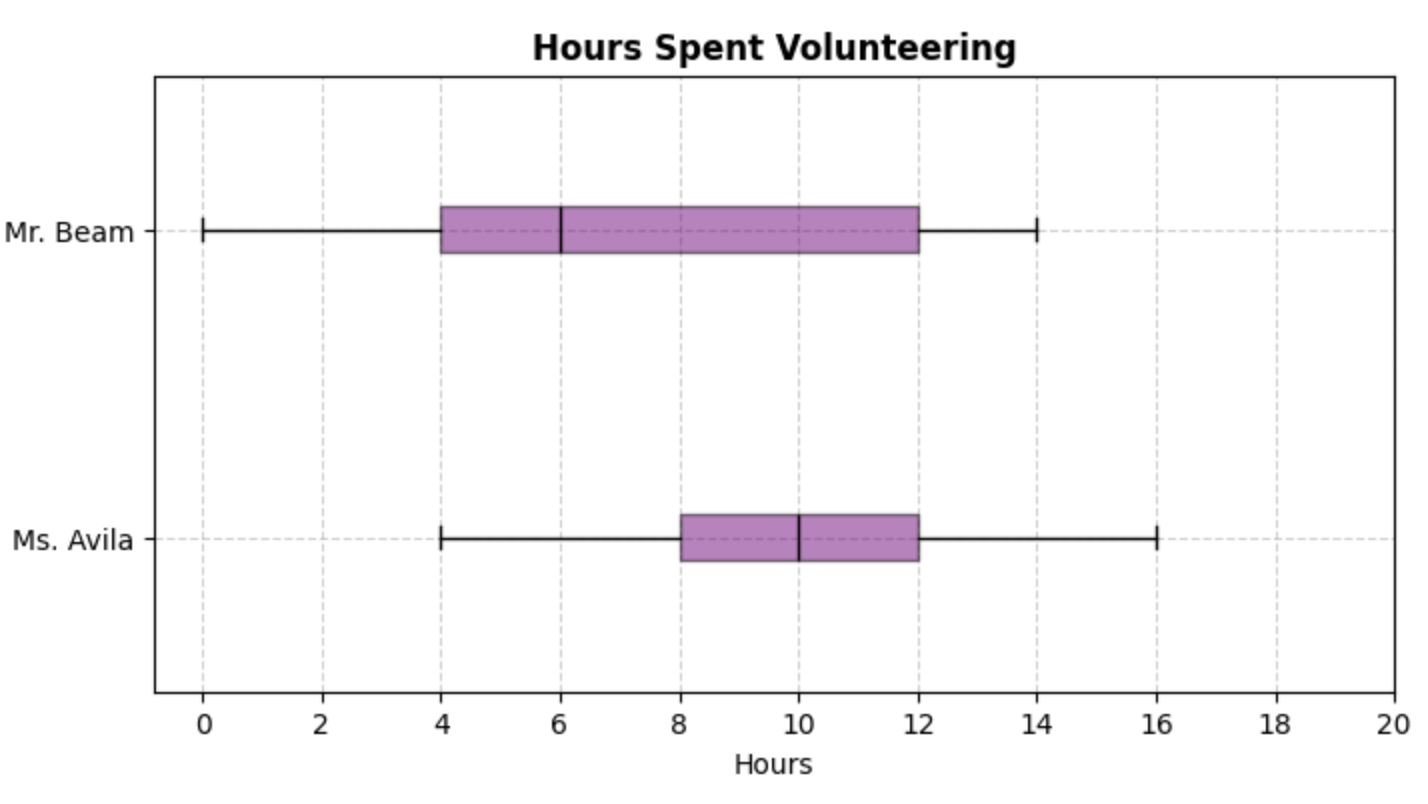
\includegraphics[width=0.8\textwidth]{F5.png}

Based on the data in the box plots, determine which statement is true?

\choicebox{A}{The student who volunteered the least number of hours is in Ms. Avila’s class.}  
\choicebox{B}{Students in Ms. Avila’s class generally spent less time volunteering than students in Mr. Beam’s class did.}  
\choicebox{C}{The IQR in the amount of time students in Ms. Avila’s class spent volunteering is less than the amount of time students in Mr. Beam’s class spent volunteering.}  
\choicebox{D}{One fourth of all the students in the two classes combined volunteered for at least 12 hours.}  



\newpage

\noindent\markforreview
\vspace{1em}

In a set of four consecutive odd integers, where the integers are ordered from least to greatest, the first integer is represented by $x$. The product of 28 and the third odd integer in the set is at most the value of 50 less than the sum of the first and fourth odd integers in the set. What is the greatest possible value of $x$?

\choicebox{A}{$-5$}  
\choicebox{B}{$-6$}  
\choicebox{C}{$-7$}  
\choicebox{D}{$-8$}  

\vspace{2em}


\noindent\markforreview
\vspace{1em}

In the given equation, $c$ is a constant. A solution to the equation is  
\[
\frac{-27 + \sqrt{261}}{26}
\]  
What is the value of $c$?

\[
x(13x + 27) + c = 5
\]

\choicebox{A}{14}  
\choicebox{B}{9}  
\choicebox{C}{5}  
\choicebox{D}{4}  

\newpage

\noindent\markforreview
\vspace{1em}

The function $h(x)$ is defined as:  
\[
h(x) = -\sqrt{x^2 + bx + c}
\]  
where $b$ and $c$ are constants. The graph of $y = h(x)$ contains the points $(2, 0)$ and $(0, -\sqrt{358})$. If $h(m) = 0$, what is the greatest possible value of $m$?

\choicebox{A}{2}  
\choicebox{B}{177}  
\choicebox{C}{179}  
\choicebox{D}{358}  

\vspace{2em}
\noindent\markforreview
\vspace{1em}

The functions \(f\) and \(g\) are defined by the equations shown, where \(a\) and \(b\) are integer constants, \(a < b\), and \(b < 0\). If \(y = f(x)\) and \(y = g(x)\) are graphed in the \(xy\)-plane, which of the following equations displays, as a constant or coefficient, the \(y\)-coordinate of the \(y\)-intercept of the graph of the corresponding function?

\begin{itemize}
    \item[I.] \(f(x) = a(2.1)^{x + b}\)
    \item[II.] \(g(x) = a(2.1)^x + b\)
\end{itemize}

\choicebox{A}{I only}  
\choicebox{B}{II only}  
\choicebox{C}{I and II}  
\choicebox{D}{Neither I nor II}

\newpage

\noindent\markforreview
\vspace{1em}

A right rectangular prism \(X\) is similar to right rectangular prism \(Y\). The surface area of right rectangular prism \(X\) is 56 square centimeters (\(\text{cm}^2\)), and the surface area of right rectangular prism \(Y\) is 896 \(\text{cm}^2\). The volume of right rectangular prism \(Y\) is 1,536 cubic centimeters (\(\text{cm}^3\)). What is the sum of the volumes, in \(\text{cm}^3\), of right rectangular prism \(X\) and right rectangular prism \(Y\)?

\vspace{0.75em}


\vspace{2em}

\noindent\markforreview
\vspace{1em}

To investigate the effect of magnesium supplementation on the sleep quality of adults, a researcher selected 190 adults at random from a community center to participate in a study. Each participant was then randomly assigned to take a magnesium supplement or a placebo each day for 6 weeks. At the end of the 6 weeks, the researcher measured the sleep efficiency of all participants again and found that the magnesium supplement caused statistically significant improved sleep quality for the adults at the community center. What feature of this study allowed the researcher to conclude that the magnesium supplement caused the improved sleep quality?

\vspace{0.75em}

\choicebox{A}{There were more than 100 participants in the study.}  
\choicebox{B}{The participants were selected at random from the community center.}  
\choicebox{C}{The sleep efficiency of each participant was measured again at the end of 6 weeks.}  
\choicebox{D}{Each participant was randomly assigned to take a magnesium supplement or a placebo.}  

\newpage
\noindent\markforreview
\vspace{1em}

For the function \(f\), for every increase of 2 in the value of \(x\), the value of \(f(x)\) increases by a factor of \(c\), where \(c\) is a constant. Which of the following equivalent forms of function \(f\) displays the value of \(c\) as the base or the coefficient?

\choicebox{A}{\(f(x) = 42(2)^{6x}\)}  
\choicebox{B}{\(f(x) = 42(8)^{2x}\)}  
\choicebox{C}{\(f(x) = 42(64)^x\)}  
\choicebox{D}{\(f(x) = 42(4{,}069)^{\frac{x}{2}}\)}






\end{document}